%LET'S GO TEAM!!! ONE LESS SECTION
%We are unstoppppable --> DAB DAB DAB


\subsection{Introduction}
% You are doing GREAT JOB!!!

The first step to build a satellite network with global coverage is to compute a single satellite footprint.\\

The footprint of a satellite is defined as the region of Earth where a single satellite can be seen. This Earth coverage surface provided is spherical and depens on some orbital paramaeters such as:

\begin{itemize}
\item Height \\
When increasing height the footprint of a satellite grows.
\item Elevation angle \\
When increasing the elevation angle, which is the angle between the satellite and the horizontal plane of an arbitrari point of the Eartg, the surface seen by the satellites descreases. (This parameter will be later studied in detail)
\end{itemize}

\subsection{Footprint Computation}
 
\begin{figure}[H] %[b] % h / H / b / t

	\centering
	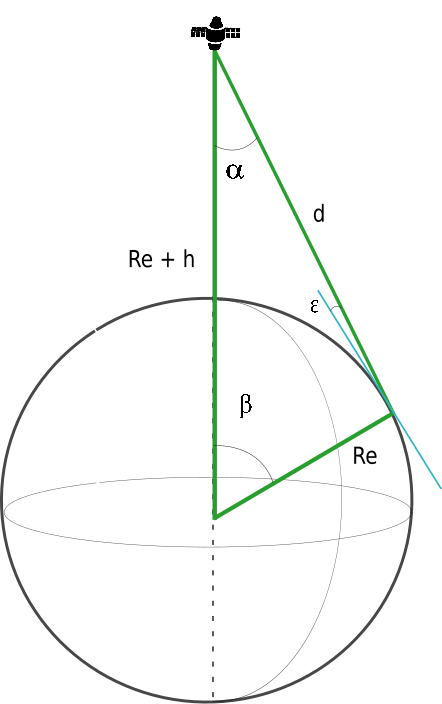
\includegraphics[width=.3\textwidth]{./fig-Ch2-OrbitalCoverage/AngleSSatFoot.png}
	\caption{Single satellite coverage geometry}
	\label{fig:AngleSSatFoot}
	
\end{figure}

 In order to compute the coverage area we must solve the triangle depicted in figure~\ref{fig:AngleSSatFoot} where the basic geometry of a satellite footprint is shown.

 The most needed parameters are the distance from a random point on Earth (where we can suppose our ground station to be) to the satellite denoted by $d$ and the central angle, denoted with a $\beta$ . \\
 
 Applying cosines law to the triangle shown in figure~\ref{fig:AngleSSatFoot}, we obtain the following expression:
 
 \begin{equation} 
\begin{gathered}
r^2=R_{earth}^2+d^2-cos(90+\epsilon)
\end{gathered}
\label{eq:Tcos}
\end{equation}
 
 Isolating $d$ from the equation above and changing $r=R_{earth}+h$, where $h$ is the actual height of the satellite regarding the Earth surface, we arrive at:
 
\begin{equation}
\begin{gathered}
d=R_{earth}\left[ \sqrt{\left(\frac{h+R_{earth}}{R_{earth}}\right)^2-cos^2\epsilon}-sin\epsilon\right]
\end{gathered}
\label{eq:solvd}
\end{equation}

From the figure~\ref{fig:AngleSSatFoot} we can also extract a relation between the central angle, the distance $d$ and the elevation angle. This relation together with the equation~\ref{eq:solvd} allow us to find $\beta$. 

\begin{equation}
\begin{gathered}
d cos\epsilon=\left(R_{earth}+h\right)sin\beta \\
\beta=\frac{1}{R_{earth}+h}\arcsin\left[d(\epsilon)cos\epsilon\right]
\end{gathered}
\label{eq:solvb}
\end{equation}

Once the central angle $\beta$ has been computed we are able to obtain the footprint satellite's are using the equetion below:

\begin{equation}
\begin{gathered}
S=2 \pi R_{earth}^2 (1-cos\beta)
\end{gathered}
\label{eq:solvS}
\end{equation}

The size of the footprint will determine the level of coverage our constellation provides, therefore when deciding the value of the orbital parameters it has to be a factor to consider.
